\chapter{Published Paper}\label{sec:papers}

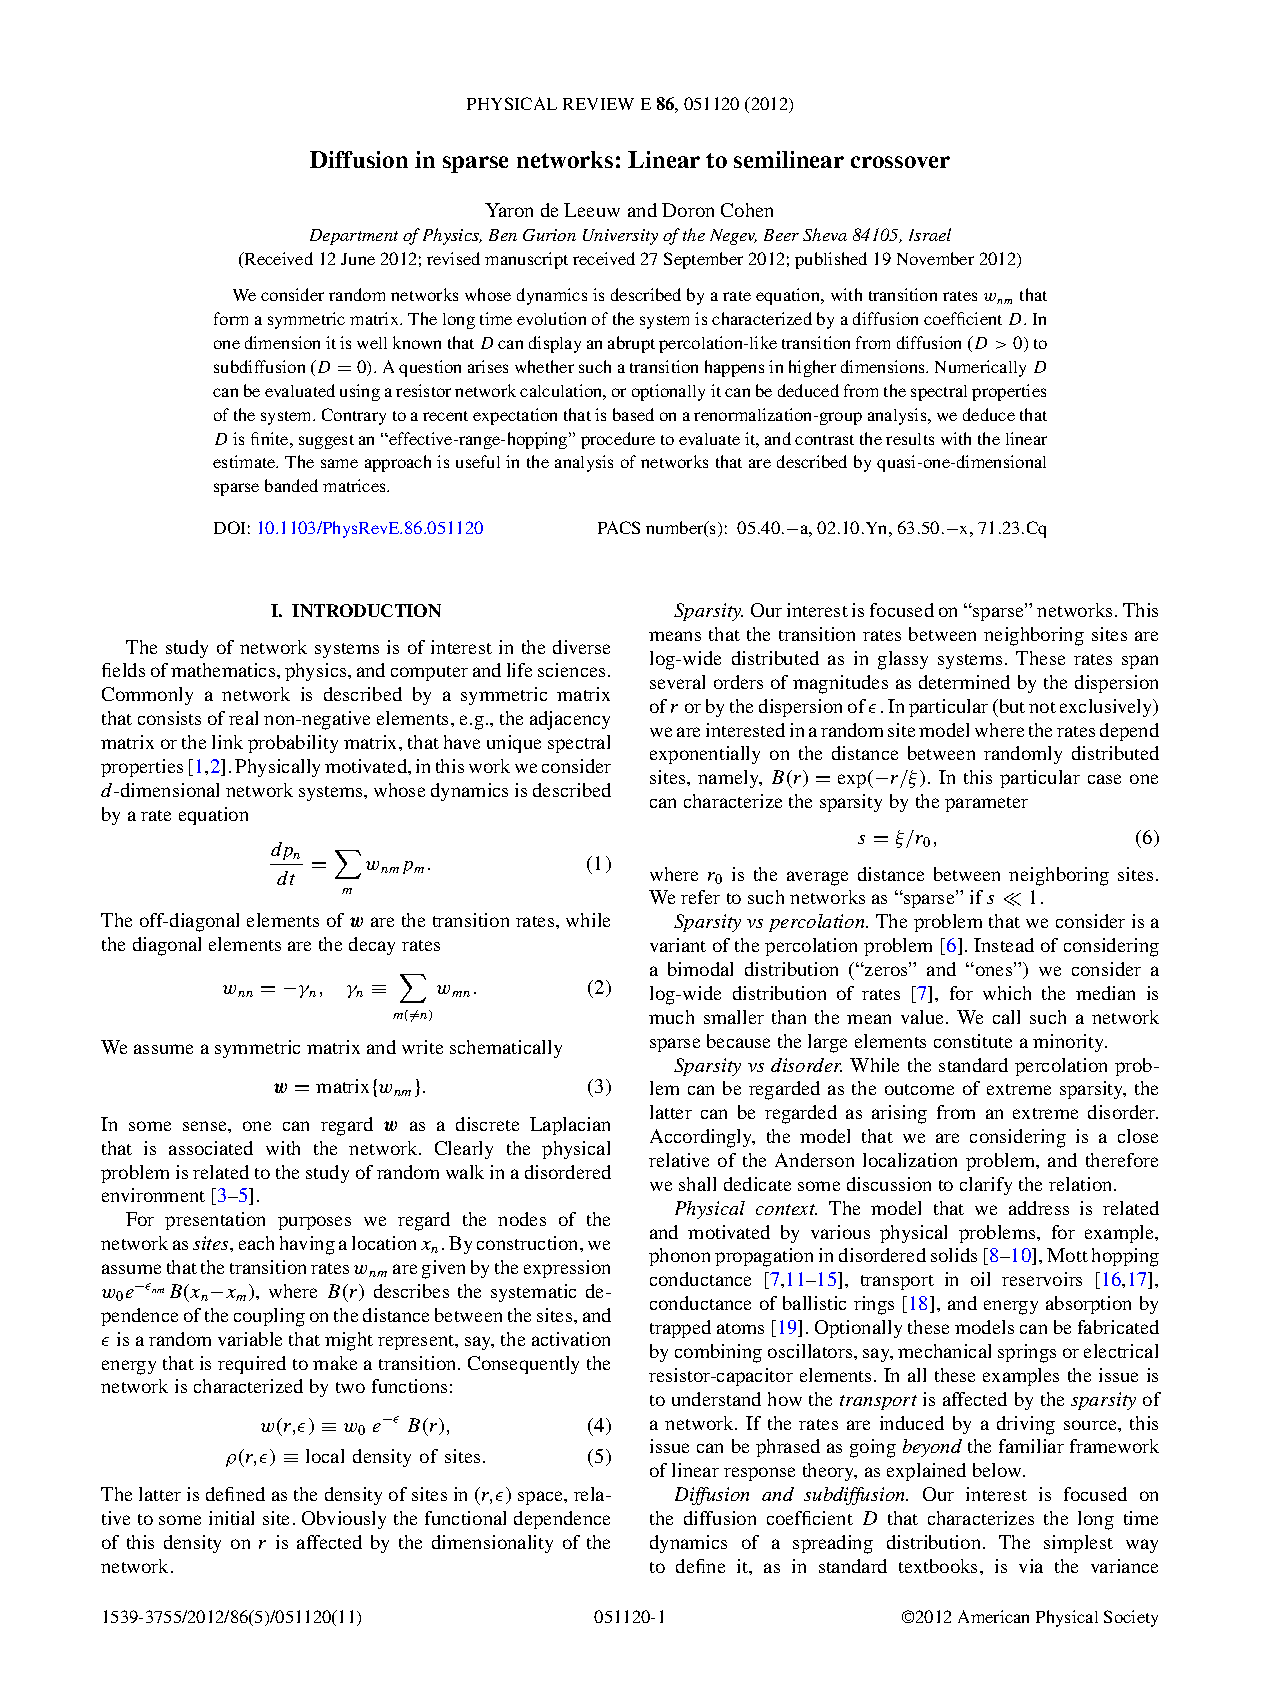
\includepdf[pages=-]{PhysRevE.86.051120.pdf}
%%%%%%%%%%%%%%%%%%%%%%%%%%%%%%%%%%%%%%%%%%%%%%
%%%%%%%%%%%%%%%%%%%%%%%%%%%%%%%%%%%%%%%%%%%%%%
\chapter{Spacing Statistics in $d$-dimensions}\label{sec:spacing}

Some clarifing points regarding the statistics of uniformly distributed sites 
will be made in this section.


There are $N$ sites distributed randomly within a $d$-dimensional
hypercube of volume $L^d$. We define a typical length $r_0$ by:
%
\begin{align}
\frac{L^d}{r_0^d} \ =\ N
\end{align}
%
From now on we shall ignore boundary conditions, assuming $N$ is large enough.
In the numerics we have used periodic boundary conditions.


If we choose some arbitrary point as the origin, the distribution of sites
around this point will be:
%
\begin{align}\label{eq:rho}
\rho(r)dr = \frac{\Omega_d r^{d-1}}{r_0^d}dr
\end{align}
% 
Where $\Omega_d$ is the $d$ dimensional solid angle:
%
\begin{align}
\Omega_d \ =\ 2,\ 2\pi,\ 4\pi, \ldots
\end{align}
%

The distribution of the nearest neighbor distance can be 
derived \cite{hertz_uber_1909,*Chandrasekhar_stochastic_1943,*Torquato_nearest-neighbor_1990},
using a differential equation. 
\rmrk{NOTE to DC: (Apparently my previous extension of the $1d$ solution to $d$ dimensions
was just a good guess, the proof is a bit less trivial then I've thought)}. %TODO remove this remark

Let us denote by $P(r)$ the probability that the first near neighbor will be
between $r$ and $r+dr$. The probability of having no neighbors up to distance $r$ is
%
\begin{align}
P_0(r) \ =\  1 - \int_0^r P(r)dr
\end{align}
$P(r)$ must equal the probability of having no neighbors up to distance $r$ times
the probabilty of finding a neighbor between $r$ and $r+dr$. So $P(r)$ must satisfy:
%
\begin{align}
P(r) \ &=\ P_0(r) \times \rho(r) \ =\ \left[ 1-\int_0^r P(r)dr \right] \rho(r) \\
\frac{P(r)}{\rho(r)}\ &=\  1-\int_0^r P(r)dr \\
\frac{d}{dr}\left(\frac{P(r)}{\rho(r)}\right) \ &=\ -\rho(r)\frac{ P(r)}{\rho(r)}
\end{align}
%
Which has the solution:
%
\begin{align}
P(r) \ &=\ \rho(r) \eexp{-\int_0^r \rho(r) dr} \\
       &=\ \frac{\Omega_d r^{d-1}}{r_0^d} \eexp{-\frac{\Omega_d}{d} \left(\frac{r}{r_0}\right)^d}  \label{eq:spacing_dist}
\end{align}
%
Where in the last step we have plugged in $\rho(r)$ from \autoref{eq:rho}
%


%The probability to have an empty surface of radius $r$ and thickness $\Delta r$
%surrounding the origin is 
%
%\begin{align}
%P_0(r<x<r+\Delta r) = (1-\rho(r)\Delta r)
%\end{align}
%
%To have an empty hypersphere, we need to have all of the surfaces empty. 
%So we can formally write $r=N\Delta r$, and multiply the probabilities:
%
%\begin{align}
%P_0(r) = \lim_{N\to \infty} \left( 1- \rho(N\Delta r)\right)^N
%\end{align}
%


%%%%%%%%%%%%%%%%%%%%%%%%%%%%%%%%%%%%%%%%%%%%%%
%%%%%%%%%%%%%%%%%%%%%%%%%%%%%%%%%%%%%%%%%%%%%%
\chapter{Resistor Network Computation}\label{sec:resnet}

%%%%%%%%%%%%%%%%%%%%%
\section{Resistor network calculation of transport}

The transmission rates of our model are analogous to
conductors. The conductance of the entire system can be derived
using Kirchoff's laws. 
We define a vector $\bm{V} = \{v_n\}$, for the voltage 
of each site (analogous to $p_n$), and a vector
$\bm{I} = \{I_n\}$ for outside current going into the site.
The Kirchoff equation takes the form
%
\begin{align}
\bm{I}\ =\ \bm{G}\cdot \bm{V}
\end{align}
%
Where $\bm{G} = \bm{W}$.


We can then add a source $I_s=-1$ and a drain $I_d=1$, setting the rest
of the currents to zero. By numerically solving the above linear equation for $\bm{V}$,
we can extract the conductivity. For practical reasons we have chosen
sites that are far away from each other but not on the edges,
and we have also looked on the voltage drop along an inner segment, to
avoid the transients at the contact points. 


In the $d{=}1$ case, the conductance is simply the conductivity multiplied
by the distance between the points.


For the $d{=}2$ case read the following section.

%%%%%%%%%%%%%%%%%%%%
\section{Point terminal resistivity in $d{=}2$}

When discussing resistivity in a square $2d$ sample, it is common
to treat two opposite edeges of the sample as terminals.
In this setting, the \emph{resistance} between the terminals equals the
\emph{resistivity} of the material. However, for our calculation,
it is easier to use point contacts as terminals. Therefore we present the
derivation of the relation between resistance and resistivity in this case.
We will assume the system is homgenous in space and as large as required.


We put a point contact source of radius $r_0$ at the origin, so 
that the current spreads to infinity with radial symmetry. The current 
density will therefore be
%
\begin{align}
J\ =\ \frac{I}{2\pi r}
\end{align}
%
The electric field and voltage are then
%
\begin{align}
E \ &=\ \rho J\ =\ \rho \frac{I}{2\pi r } \\
V \ &=\ \int_{r_0}^r E dr' \ =\ \rho\frac{I}{2\pi}\ln \frac{r}{r_0}
\end{align}
%
Here $\rho$ stands for the resistivity. We now use superposition to add a sink of radius $r_0$ at distance $r$ 
from the origin. Due to the symmetry of the problem, the voltage just doubles. The resistance is now:
%
\begin{align}
R \ &=\ \frac{V}{I}\ =\ \frac{\rho}{\pi} \ln\frac{r}{r_0} \\
\rho \ &= \ \frac{\pi}{\ln\frac{r}{r_0}} \ R
\end{align}
%
In order to find $\rho$ we compute $R$ numerically.


%%%%%%%%%%%%%%%%%%%%%%%%%%%%%%%%%%%%%%%%%%%%%%%%%%%%%%%%%%%%%%%%%%%%%%
\chapter{Numerical Routines}

For the numerical calculations, we have used python 2.6 \cite{guido_van_rossum_python_????}, together
with the scipy \cite{jones_scipy:_2001} package for numerics and the matplotlib \cite{hunter_matplotlib:_2007} package
for graphics. The source files are available online at : 
\url{http://physweb.bgu.ac.il/~jarondl/LINKS/MSc_FILES/}.


The source files are packaged into a standard python package,
and can be installed as any other package. If a package manager is installed (e.g.\ pip),
one should use it, as in :
\begin{verbatim}
pip install --user http://physweb.bgu.ac.il/~jarondl/LINKS/MSc_FILES/jarondl_msc-1.0.tar.gz
\end{verbatim}
If not, the package should be extracted, and the "setup.py" script can be used:
\begin{verbatim}
python setup.py install --user
\end{verbatim}
After this installation, the jarondl\_msc package will be available,
including the following modules:
\begin{verbatim}
ptsplot  geometry  plotdl  sparsedl
\end{verbatim}

The \texttt{ptsplot} module is the main file of the package. The three other files contain
sub-routines and class defentions used in \texttt{ptsplot}.


To reproduce all of the plots used in this proposal, one can simply run:
\begin{verbatim}
python -m jarondl_msc.ptsplot
\end{verbatim}
If the files \texttt{D\_banded.npz, D\_banded\_b10.npz } and \texttt{D\_2d.npz} (available online)
exist in the same directory as where the script is run,
this data will be used. Otherwise, the numerics will run first, and then the plots will be made. This might take several hours,
depending on the computer.



